\section{General Scene Recognition Outline}\label{section:placeOutline}

After the data are fused into a uniform scene representation, the scene recognition is performed. This algorithm aims to remember all scenes the robot has visited and to decide if the current scene, received from the sensors, has been already visited or not, and eventually return the unique identification of the previously visited scene.\par
In order to achieve this goal, we need to find a suitable representation (further template) of the scene that will be remembered by the robot. This template must be created from the fused scene description received from the sensors, should occupy little space, and be easy to compare.\par
The scene recognition algorithm works in three steps. In the first step, the designed template is built from the received fused scene representation. In the second step, this template is independently compared with all the stored templates, representing previously visited scenes. A template comparison result is a real number between 0 and 1, representing the similarity of both templates. The closer the similarity to 1, the more similar the templates are. After all the templates are compared, the most similar template is chosen. In the last step, the similarity of the most similar template is compared to the given threshold. If it is greater, the most similar template is returned as the same scene. If it is smaller, the current template will be remembered, and the result will be that this scene was not visited before. The whole process is visualized in Figure \ref{fig:placeRecognitionWorkflow}.\par

\begin{figure}[htpb]
    \centering
    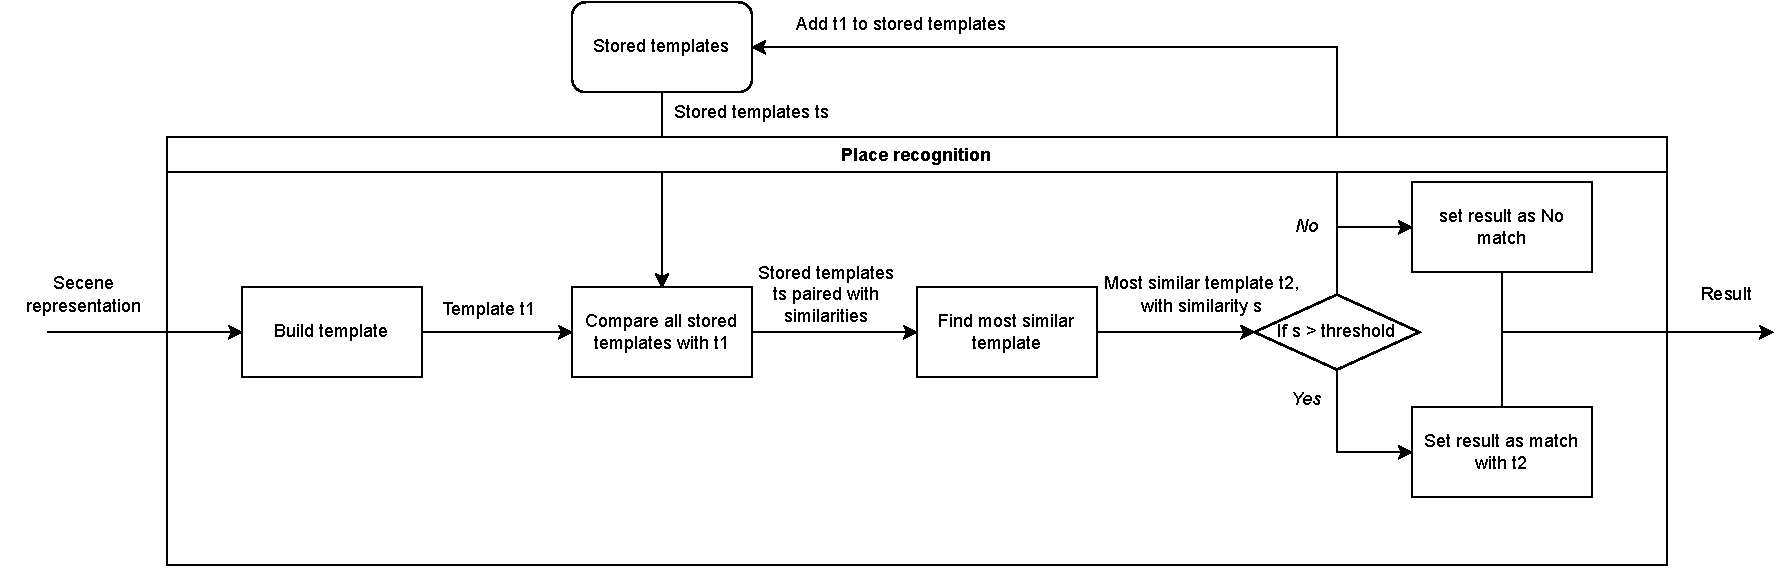
\includegraphics[width=1\textwidth]{placeRecognitionWorkflow.pdf}
    \caption{Common scene recognition workflow} \label{fig:placeRecognitionWorkflow}
\end{figure}

The following sections suggest three different approaches to scene recognition. All presented techniques differ in template structures and template building and comparison algorithms. Otherwise, they all share the same structure shown in this section.